\let\negmedspace\undefined
\let\negthickspace\undefined
\documentclass[report]{IEEEtran}
\usepackage[a5paper, margin=10mm, onecolumn]{geometry}
%\usepackage{lmodern} % Ensure lmodern is loaded for pdflatex
\usepackage{tfrupee} % Include tfrupee package

\setlength{\headheight}{1cm} % Set the height of the header box
\setlength{\headsep}{0mm}     % Set the distance between the header box and the top of the text

\usepackage{gvv-book}
\usepackage{gvv}
\usepackage{cite}
\usepackage{amsmath,amssymb,amsfonts,amsthm}
\usepackage{algorithmic}
\usepackage{graphicx}
\usepackage{textcomp}
\usepackage{xcolor}
\usepackage{txfonts}
\usepackage{listings}
\usepackage{enumitem}
\usepackage{mathtools}
\usepackage{gensymb}
\usepackage{comment}
\usepackage[breaklinks=true]{hyperref}
\usepackage{tkz-euclide} 
\usepackage{listings}
% \usepackage{gvv}                                        
\def\inputGnumericTable{}                                 
\usepackage[latin1]{inputenc}                                
\usepackage{color}                                            
\usepackage{array}                                            
\usepackage{longtable}                                       
\usepackage{calc}                                             
\usepackage{multirow}                                         
\usepackage{hhline}                                           
\usepackage{ifthen}                                           
\usepackage{lscape}
\begin{document}

\bibliographystyle{IEEEtran}
\vspace{3cm}

\title{EE1200 - ELECTRIC CIRCUITS LAB }
\author{EE24BTECH11012 - Bhavanisankar G S \\ EE24BTECH11019 - Dwarak A}
% \maketitle
% \newpage
% \bigskip
{\let\newpage\relax\maketitle}

\renewcommand{\thefigure}{\theenumi}
\renewcommand{\thetable}{\theenumi}
\setlength{\intextsep}{10pt} % Space between text and floats
\section{Plot at least 6 Lissajous figures and justify the pattern you see on CRO, with theory.}

\subsection{AIM : }
To plot at least 6 Lissajous figures and justify the pattern seen on CRO.

\subsection{Apparatus Required : }
\begin{itemize}
    \item An Oscilloscope
    \item A function generator
    \item Power supply
    \item A probe
    \item Connecting wires
    \item A device to capture the image
\end{itemize}

\subsection{Theory : }
\begin{enumerate}
    \item An \color{blue} oscilloscope \color{black} is an electronic instrument that graphically displays varying signal voltages, typically as a two-dimensional plot with time on the horizontal axis and voltage on the vertical axis. 
    \item It allows for the visualization of electrical signals and helps analyze waveform properties like amplitude, frequency, and phase.
    \item A \color{blue} function generator \color{black} is a device that produces various periodic waveforms, such as sine, square, and triangular waves, across a range of frequencies. 
    \item It is used to provide the input signals required for experiments involving wave behavior.
    \item \color{blue} Lissajous figures \color{black} are complex patterns that result from the combination of two perpendicular sinusoidal signals with varying frequency and phase. They are described mathematically as:
    \begin{align}
        x(t) &= A \sin \brak{at + \delta} \\
        y(t) &= B \sin \brak{bt}
    \end{align}
    where, 
    \begin{align*}
        A, B &- \text{ Amplitudes } \\
        a, b &- \text{ Angular frequencies } \\
        t &- \text{ Time }\\
        \delta &- \text{ Phase difference }
    \end{align*}
    \item For generating Lissajous figures, the function generator produces two sinusoidal signals with adjustable frequency and phase difference.
    \item The oscilloscope operates in $XY$ mode, where one input signal is applied to the horizontal (X) axis and another to the vertical (Y) axis. This mode visualizes the relationship between two signals rather than plotting voltage versus time.
    \item The shape of the Lissajous figure depends on the ratio \( \frac{a}{b} \) and the phase difference \( \delta \):

\begin{itemize}
    \item \textbf{Equal Frequencies} (\( a = b \)): The figure appears as an ellipse, circle, or straight line, depending on the phase difference.
    
    \item \textbf{Frequency Ratio} \(\left( \frac{a}{b} = \frac{n}{m} \right)\): Closed, symmetric patterns form when the ratio is rational.
    
    \item \textbf{Phase Difference} (\( \delta \)): Determines the orientation and complexity of the figure. \\
\end{itemize}
    \item Using the trigonometric identity for the sine of a sum:
\begin{align*}
    \sin(a t + \delta) = \sin(a t) \cos(\delta) + \cos(a t) \sin(\delta)
\end{align*}

Substituting into $x(t)$:
\begin{align*}
    x(t) &= A [\sin(a t) \cos(\delta) + \cos(a t) \sin(\delta)]
\end{align*}

\textbf{Assuming $a = b$}, let:
\begin{align*}
    u &= \sin(a t) = \frac{y}{B}, \\
    v &= \cos(a t) = \sqrt{1 - \left(\frac{y}{B}\right)^2}
\end{align*}

Substituting back:
\begin{align*}
    x &= A \left[\frac{y}{B} \cos(\delta) + \sqrt{1 - \left(\frac{y}{B}\right)^2} \sin(\delta)\right]
\end{align*}

Squaring and rearranging gives the general form:
\begin{align*}
    \frac{x^2}{A^2} + \frac{y^2}{B^2} - \frac{2xy}{AB} \cos(\delta) = \sin^2(\delta)
\end{align*}
\textbf{For general frequency ratio \( \frac{a}{b} = \frac{n}{m} \)}, we can express the relationship using as : \\
\begin{align*}
    \cos\left(\frac{n}{a} \arcsin\left(\frac{x}{A}\right) - \delta\right) = \cos\left(\frac{m}{b} \arcsin\left(\frac{y}{B}\right)\right)
\end{align*}
\end{enumerate}

\subsection{Procedure : } \\
\begin{enumerate}
    \item Connect the function generator's output to oscilloscope channel 1 and channel 2 (ensure perpendicular signals).
    \item Set oscilloscope’s time base and voltage scale appropriately.
    \item Configure the function generator by setting channel 1 to \( f_1 \) sine wave and channel 2 to \( f_2 \) sine wave, with phase shift (\( \Delta \phi \)).
    \item Lissajous figures are formed on the oscilloscope screen.
    \item Adjust frequency ratio and phase shift, observe the changes in the figure.
    \item Frequencies, phase shifts are recorded and Observed figures are sketched.
    \item Experimental figures and Theoretical predictions are compared.
\end{enumerate}

\subsection{Figure(s) : }
            \begin{figure}[h]
    \centering
    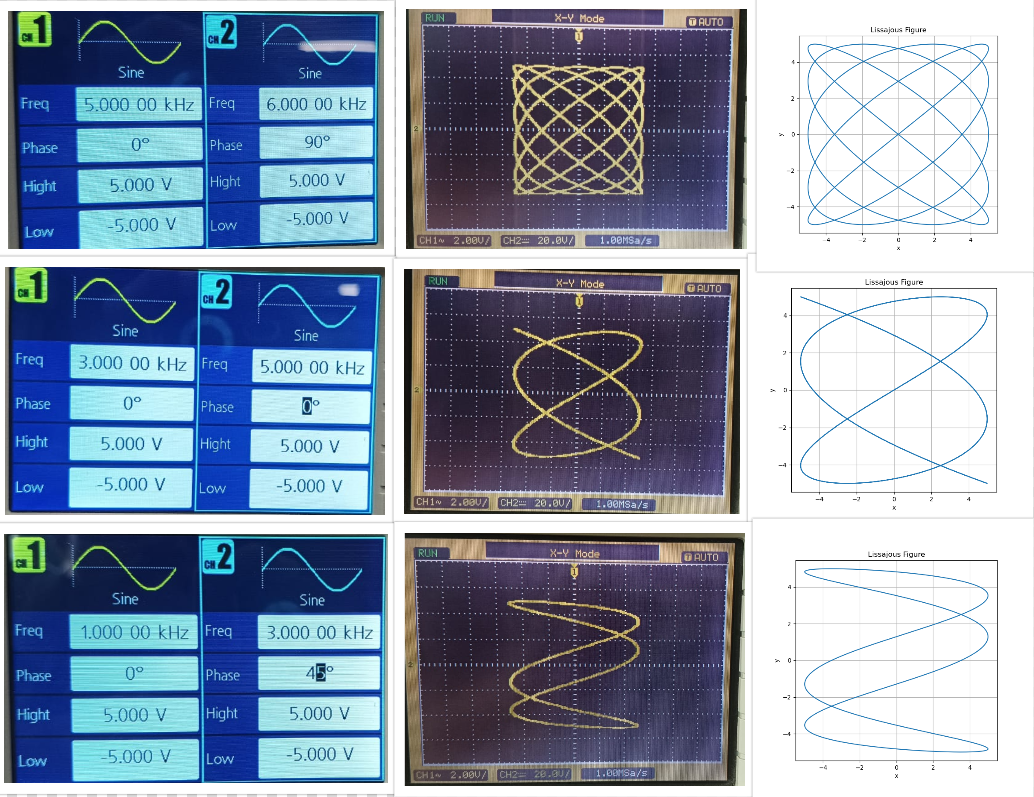
\includegraphics[width=\columnwidth]{Fig1.png}
    \label{fig:Plot1}
\end{figure}

\begin{figure}[h]
    \centering
    \begin{minipage}{\textwidth}
        \centering
        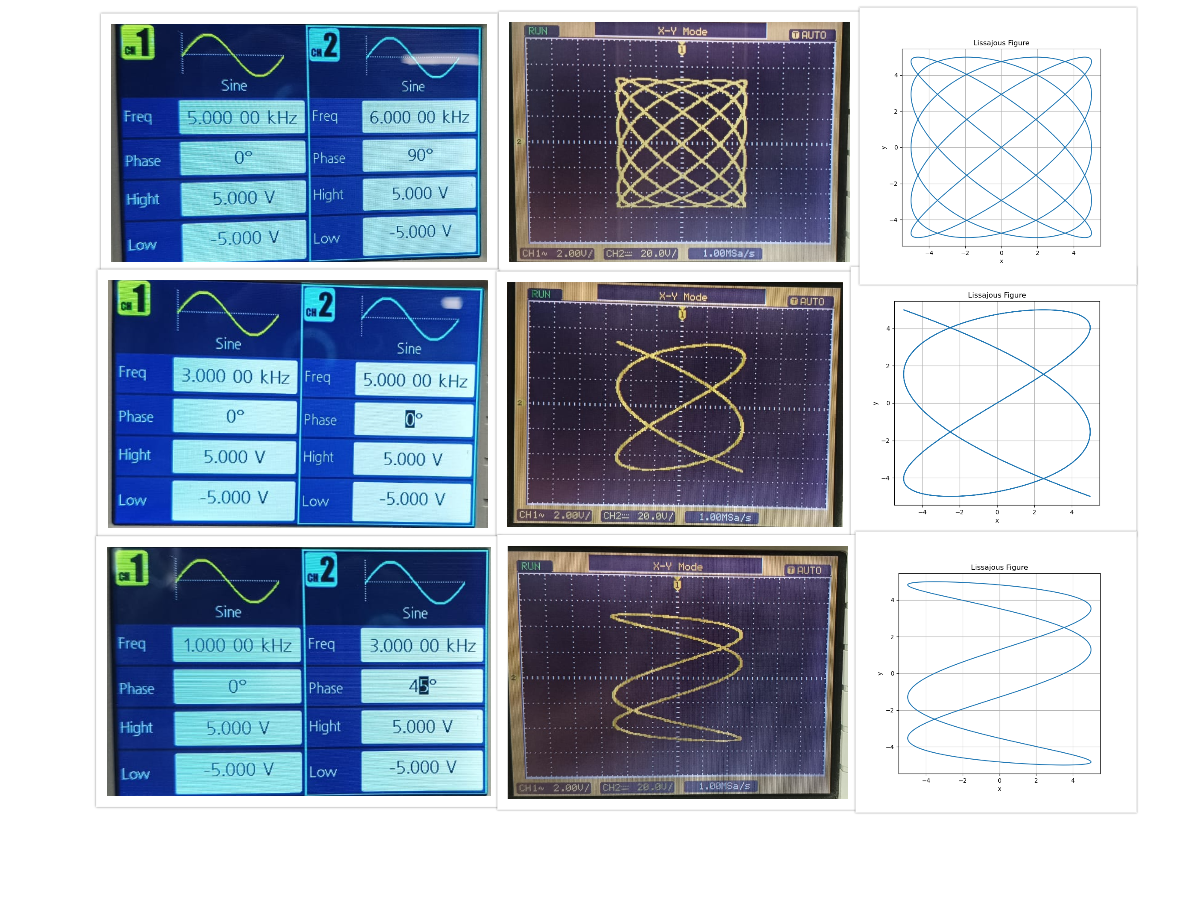
\includegraphics[width=\columnwidth]{Fig2.png}
        \label{fig:Plot2}
    \end{minipage}

    \vspace{0.5cm} % Adjust the spacing between the figures if needed

    \begin{minipage}{\textwidth}
        \centering
        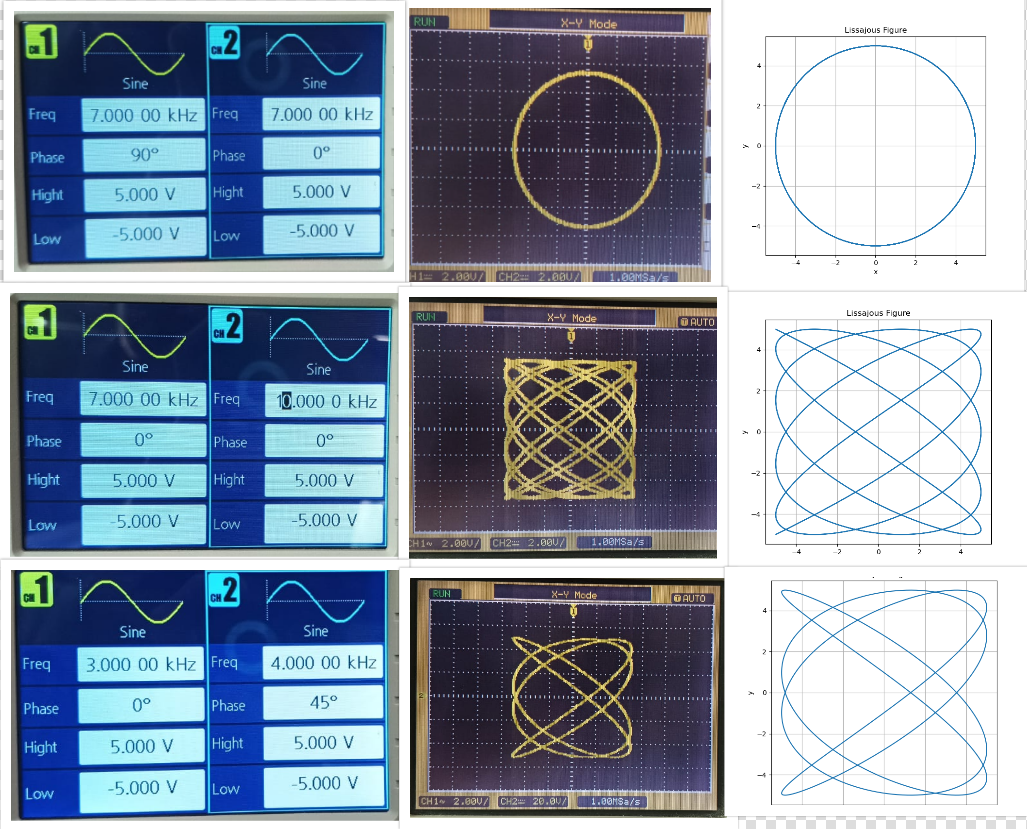
\includegraphics[width=\columnwidth]{Fig3.png}
        \label{fig:Plot3}
    \end{minipage}
\end{figure}

\newpage
\section{How do you capture a one-time event on CRO - show with an example.}

\subsection{AIM : } \\
To capture a one-time event on CRO.

\subsection{APPARATUS REQUIRED : } \\
\begin{itemize}
	\item Oscilloscope
	\item Digital Function generator
	\item A probe
	\item Connecting wires
	\item BNC cables
\end{itemize}

\subsection{Theory : } \\
\begin{itemize}
\item A \color{blue} function generator \color{black} is an electronic device that generates various types of electrical waveforms over a range of frequencies. The most common waveforms produced by a function generator are sine, square, and triangular waves. These waveforms are used to simulate signals in electronic testing and development. The function generator allows the user to adjust the frequency, amplitude, and shape of the waveform, making it a versatile tool in electronics labs.
\item An \color{blue} oscilloscope \color{black} is an electronic test instrument that graphically displays varying signal voltages, usually as a two-dimensional plot of one or more signals as a function of time. The oscilloscope can be used to observe the amplitude, frequency, and shape of the signal waveforms. It captures real-time events by continuously sampling the input signal and displaying it on the screen. Oscilloscopes are essential for diagnosing and troubleshooting electronic circuits, as they provide a visual representation of how signals behave over time.
\item \color{blue} Burst mode \color{black} in a digital function generator refers to a feature that allows the generation of a specific number of cycles of a waveform, followed by a period of no output. This mode is particularly useful for testing circuits that need to respond to a controlled, finite sequence of pulses or cycles.
\item When the \color{blue} SINGLE mode \color{black} is selected, the oscilloscope arms itself to capture a single waveform based on a specified trigger condition. Once the trigger condition is met, the oscilloscope records the waveform and then stops further acquisitions.

\end{itemize}

\subsection{PROCEDURE : } \\
\begin{itemize}
	\item Connect the digital function generator and the oscilloscope using BNC cables and a probe.
	\item Use the function generator in \color{blue} BURST \color{black} mode.
	\item Set the amplitude, frequency and the number of cycles to be captured in the function generator.
	\item Set the mode coupling to normal, run control to single in the oscilloscope and push the manual trigger in the function generator.
	\item A real-time capture of the function input can be seen on the oscilloscope display.
\end{itemize}

\subsection{FIGURES : } \\

\begin{figure}[h]
				 \centering
				 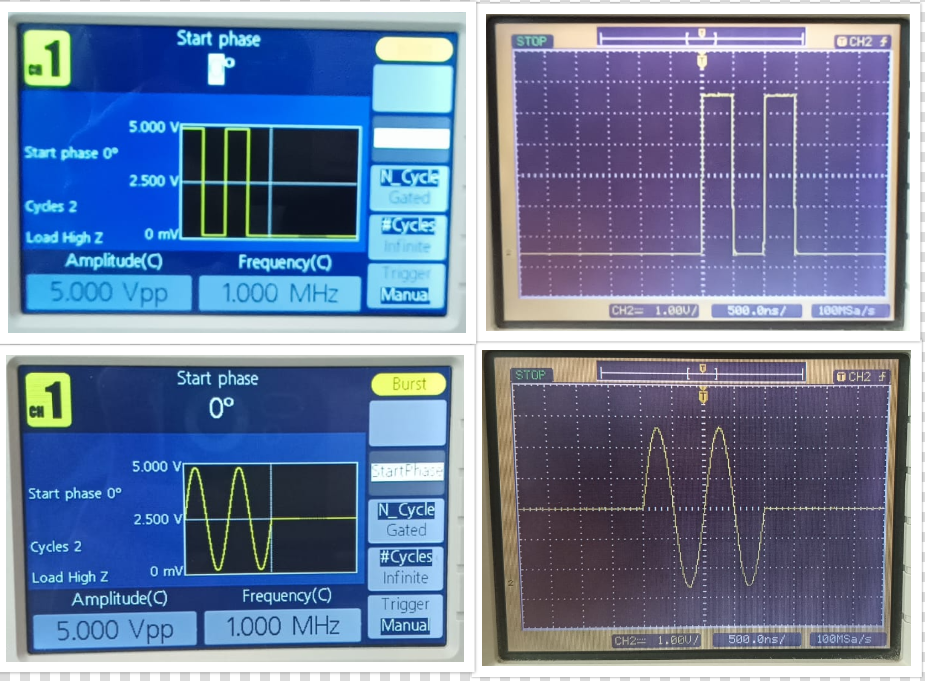
\includegraphics[width=\columnwidth]{fig1.png}
				 \label{fig:Plot1}
			 \end{figure}

\end{document}

